\section{Data selection}
\label{sec:dsphi:sel}

%LIST
%
%Rely on HLT2 tolo lines
%cuts designed to mimic HLT1 and HL2 topo triggers:
%B
%sum pt $>$ 5\gev
%VHI2DOF $<$ 10
%BPVIPCHI2 $<$25
%BPVLTIME$>$0.2\ps
%BIRA$>$0.999
%
%D
%sum PT $>$1.8GeV
%MAXDOCA$<$0.5mm
%VCHI2DOF $<$10
%BPVVDCHI2$>$36
%
%D tracks
%TRCHI2<4
%PT>100MeV
%P>1Gev
%MIPCHI2>4
%DLL<20()-10)
%
%phi
%sumPT>1
%VCHI2DOF<16
%BPVVDCHI2>16
%
%phi tracks
%TRCHI2<4
%PT>100MeV
%P>2GEv
%DLL<20()-10)
%
%Min one track \& two...


The data sample used in this analysis is the
$1\invfb$ collected by the \lhcb detector in 2011 from $pp$
collisions with a centre-of-mass energy of $7\tev$.
Events are selected if they fulfil {\tt L0Hadron TOS} or {\tt L0Global TIS}, trigger requirements.
Further trigger requirements are applied at the \hlttwo level, where events are required to pass at
least one of the hadronic topological triggers (see \Sec{sec:lhcb:trig} for more details) with {\tt TOS}.

Candidate \phii mesons are reconstructed from the decay mode \phitokk, and are only accepted if the
invariant \kk mass, $m_\kk$, is within $40\mev$ of the known \phii mass~\cite{PDG2012}
--- this is extremely loose in order to be able to constrain background components.
The \Ds meson is only reconstructed from the Cabibbo favoured decay \dstokkpi, and the candidate
mass, $m_\kkpi$, must fall within $25\mev$ of the nominal \Ds mass~\cite{PDG2012} and lie
downstream of the \Bp vertex.
All tracks forming the candidate particles must fulfill requirements on the transverse momentum,
$\pt>100\mev$, and tracks from the \Ds(\phii), $p>1(2)\gev$.
Geometrical constraints are also placed on the tracks.
The \chisq per degree of freedom of the track fit, $\chisqtrk/\ndof$, must be less than four, and
$\min\left(\chisqip\right)>4$.
The variable \chisqip is defined as the increase in \chisqvtx when the signal track is combined
with the PV; the $\min\left(\chisqip\right)$ is the minimum \chisqip with respect to all PVs.
Loose PID requirements are also placed on the tracks in order to reduce the retention rate of the
stripping line.

The \Bp vertex fit is performed by constraining the mass of the \Ds to its known
mass~\cite{PDG2012}, and the resulting vertex fit must have a \chisqvtx per degree of freedom of
less than ten.
The angle between the vector formed by the PV and \Bp decay vertex and the vector formed by the
momentum of all the daughter tracks is the direction angle, \thetadir.
Were the resolution of the \lhcb detector to be perfect, a real decay would have $\cos\thetadir=1$,
for this analysis a constraint of $\cos\thetadir>0.999$ is applied.
In order to remove prompt background from the PV, the lifetime of the \Bp, $\tau_{\Bp}$, must be
greater than $0.2\ps$.
Cuts applied in the stripping selection are summarized in \Tab{tab:dsphi:sel}.


%Candidate \Ds and \phii mesons are reconstructed only in the decays \decay{\Ds}{\kkpi} and
%\phitokk, where the \Ds decay is the Cabibbo favoured mode.
%Each daughter track has a $\chisqtrk/\ndof<4$, a \pt of at least $100\mev$, and a minimum momentum
%of $1$ or $2\gev$ for tracks originating from the \Ds and \phii, respectively.
%Each track in the event must also be detached from the PV, and are only accepted if the
%$\chisqvtx/\ndof$ increases by more than four when the track is used in the vertex fit, compared to
%when it is omitted.
%Very loose PID requirements are also placed on the tracks, this is more to reduce the rate of the
%stripping line that to identify pions and kaons, this is done later in the selection process.
%
%The \Ds and \phii are also subject to requirements on the \chisq of the vertex separation,
%\chisqvs, which is tighter for the \Ds because of its finite lifetime.
%Full stripping requirements are given in \Tab{tab:dsphi:sel}.

\begin{table}[!ht]
  \caption[Selection of \btodsphi candidates.]
  {\small
    Selection applied to the \btodsphi candidates.
    The DOCA variable is defined as the maximum distance of closest approach between all pairs of
    all pairs of daughter particles.
    All remaining variables are defined in the text.
  }
  \label{tab:dsphi:sel}
  \begin{center}
    \begin{tabular}{cccc}
      \toprule
      Candidate & \multicolumn{3}{c}{Cut} \\
      \midrule
      \Bp
      %\multirow{5}{*}{\Bp}
      & $\sum p_T^\mathrm{tracks}$ &$>$& $5\gev$ \\
      & \chisqvtx/\ndof &$<$& 10 \\
      & \chisqip &$<$& 25 \\
      & $\tau$ &$>$& $0.2\ps$ \\
      & $\cos\thetadir$ &$>$& $0.999$ \\
      %& $\bdt_\mathrm{strip}$ &$>$& 0.05 \\
      \littlerule
      \Ds
      %\multirow{3}{*}{\Ds}
      & $\sum p_T^\mathrm{tracks}$ &$>$& $1.8\gev$ \\
      & \chisqvtx/\ndof &$<$& 10 \\
      & DOCA &$<$& $0.5\mm$ \\
      \littlerule
      Tracks from \Ds
      %\multirow{6}{*}{Tracks from \Ds}
      & \pt &$>$& $100\mev$ \\
      & $p$ &$>$& $1\gev$ \\
      & $\chisqtrk/\ndof$ &$<$& $4$ \\
      & $\min\!\left(\chisqip\right)$ &$>$& $4$ \\
      %& \chisqvs &$>$& 36 \\
      & $\dllkpi(K)$ &$>$& $-10$ \\
      & $\dllkpi(\pi)$ &$<$& $20$ \\
      \littlerule
      \phii
      %\multirow{2}{*}{$\phi$}
      & $\sum\pt^\mathrm{tracks}$ &$>$& $1\gev$ \\
      & \chisqvtx/\ndof &$<$& 16 \\
      \littlerule
      Tracks from $\phi$
      %\multirow{4}{*}{Tracks from $\phi$}
      & \pt &$>$& $100\mev$ \\
      & $p$ &$>$& $2\gev$ \\
      & $\chisqtrk/\ndof$ &$<$& $4$ \\
      & $\min\!\left(\chisqip\right)$ &$>$& $4$ \\
      %& \chisqvs &$>$& 16 \\
      %\midrule
      %STUFF FOR 1 AND 2 TRACKS
      \bottomrule
    \end{tabular}
  \end{center}
\end{table}


%After the stripping selection, further cuts are applied.
%The invariant mass of the \Ds candidates are required to be within $25\mev$j
%its nominal value cited in \Ref{PDG2012}.
%Cuts are also applied to reconstructed \phii mass, this is described later, in \Sec{sec:dsphi:hel}.
%The decay vertex of the \Ds is required to be downstream of the decay vertex of the \Bp, and the
%$p$-value formed from the sum of the \chisqip and \chisqvtx of the \Bp candidate is also required
%to be greater than $0.1\pc$.
%Charmless backgrounds are suppressed by requiring that the \chisqfd from the \Bp vertex was greater
%than two.





There is potential for cross-feed from the decay \decay{\Dp}{\Km\pip\pip} and
the signal \Ds final state if one of the \pip{s} is misidentified as a \Kp.
The resulting invariant \kkpi combination --- with one kaon being a misidentified pion --- may fall
within $25\mev$ of the nominal \Ds mass.
%This is possible because the \Ds is approximately $100\mev$ heavier than the \Dp.
Similarly, there is potential contamination from the decay \decay{\Lc}{p\Km\pip}.
These two modes of cross-feeds are suppressed by a series of conditions.
Firstly, if the mass of the \kk pair from the \Ds decay is within $10\mev$ of the \phii mass, then
the candidate is accepted as coming from the decay \decay{\Ds}{\kkpi}.
Otherwise, a track is assigned the mass of a pion or proton, so as the new object is consistent
with a \kkpi or $p\Km\pip$, respectively.
If the invariant mass of this newly reconstructed object falls within the nominal mass of the \Dp
or \Lc, then the ambiguous (swapped) track is subject to the stringent PID requirements of
$\dllkpi>10$ or $\dllkp>0$, respectively.



\begin{figure}
  \begin{center}
    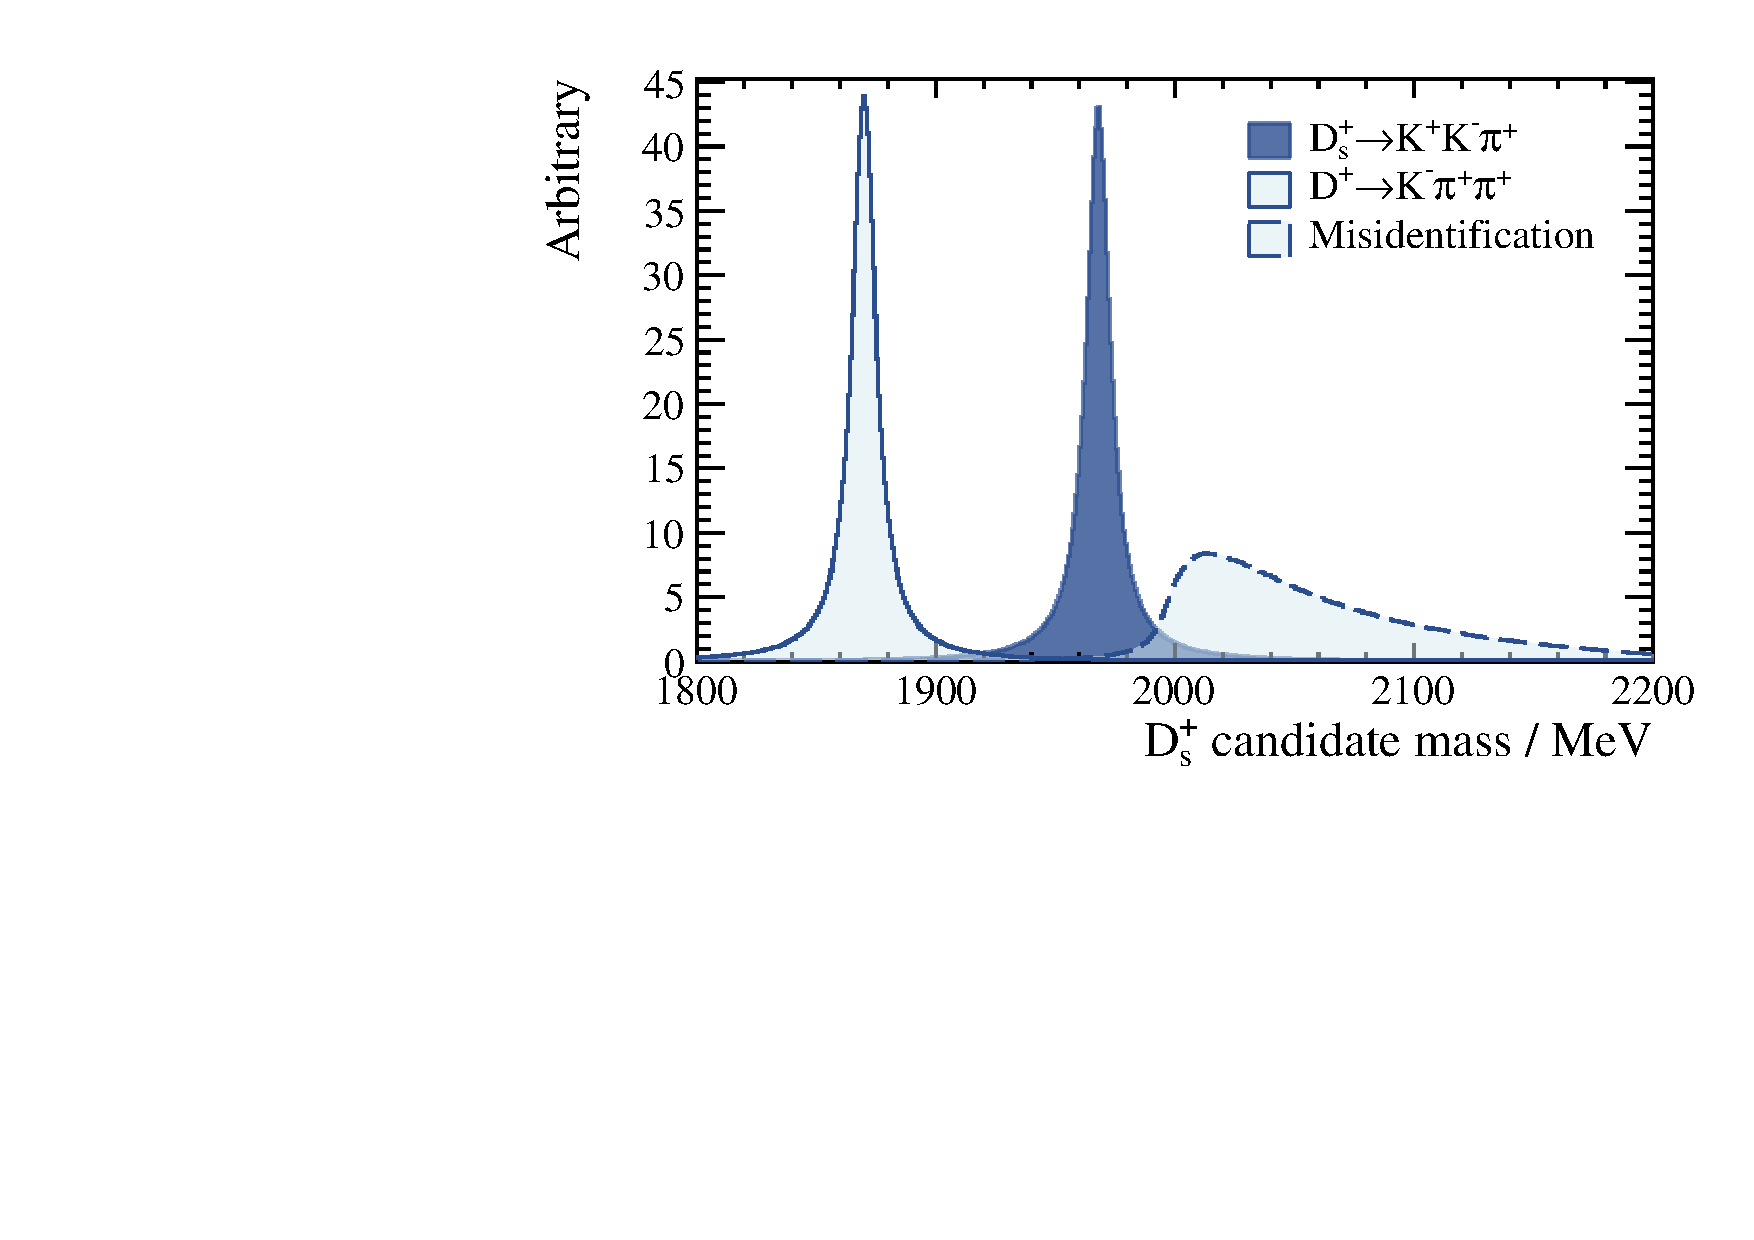
\includegraphics[width=0.48\textwidth]{tgen_dveto}
    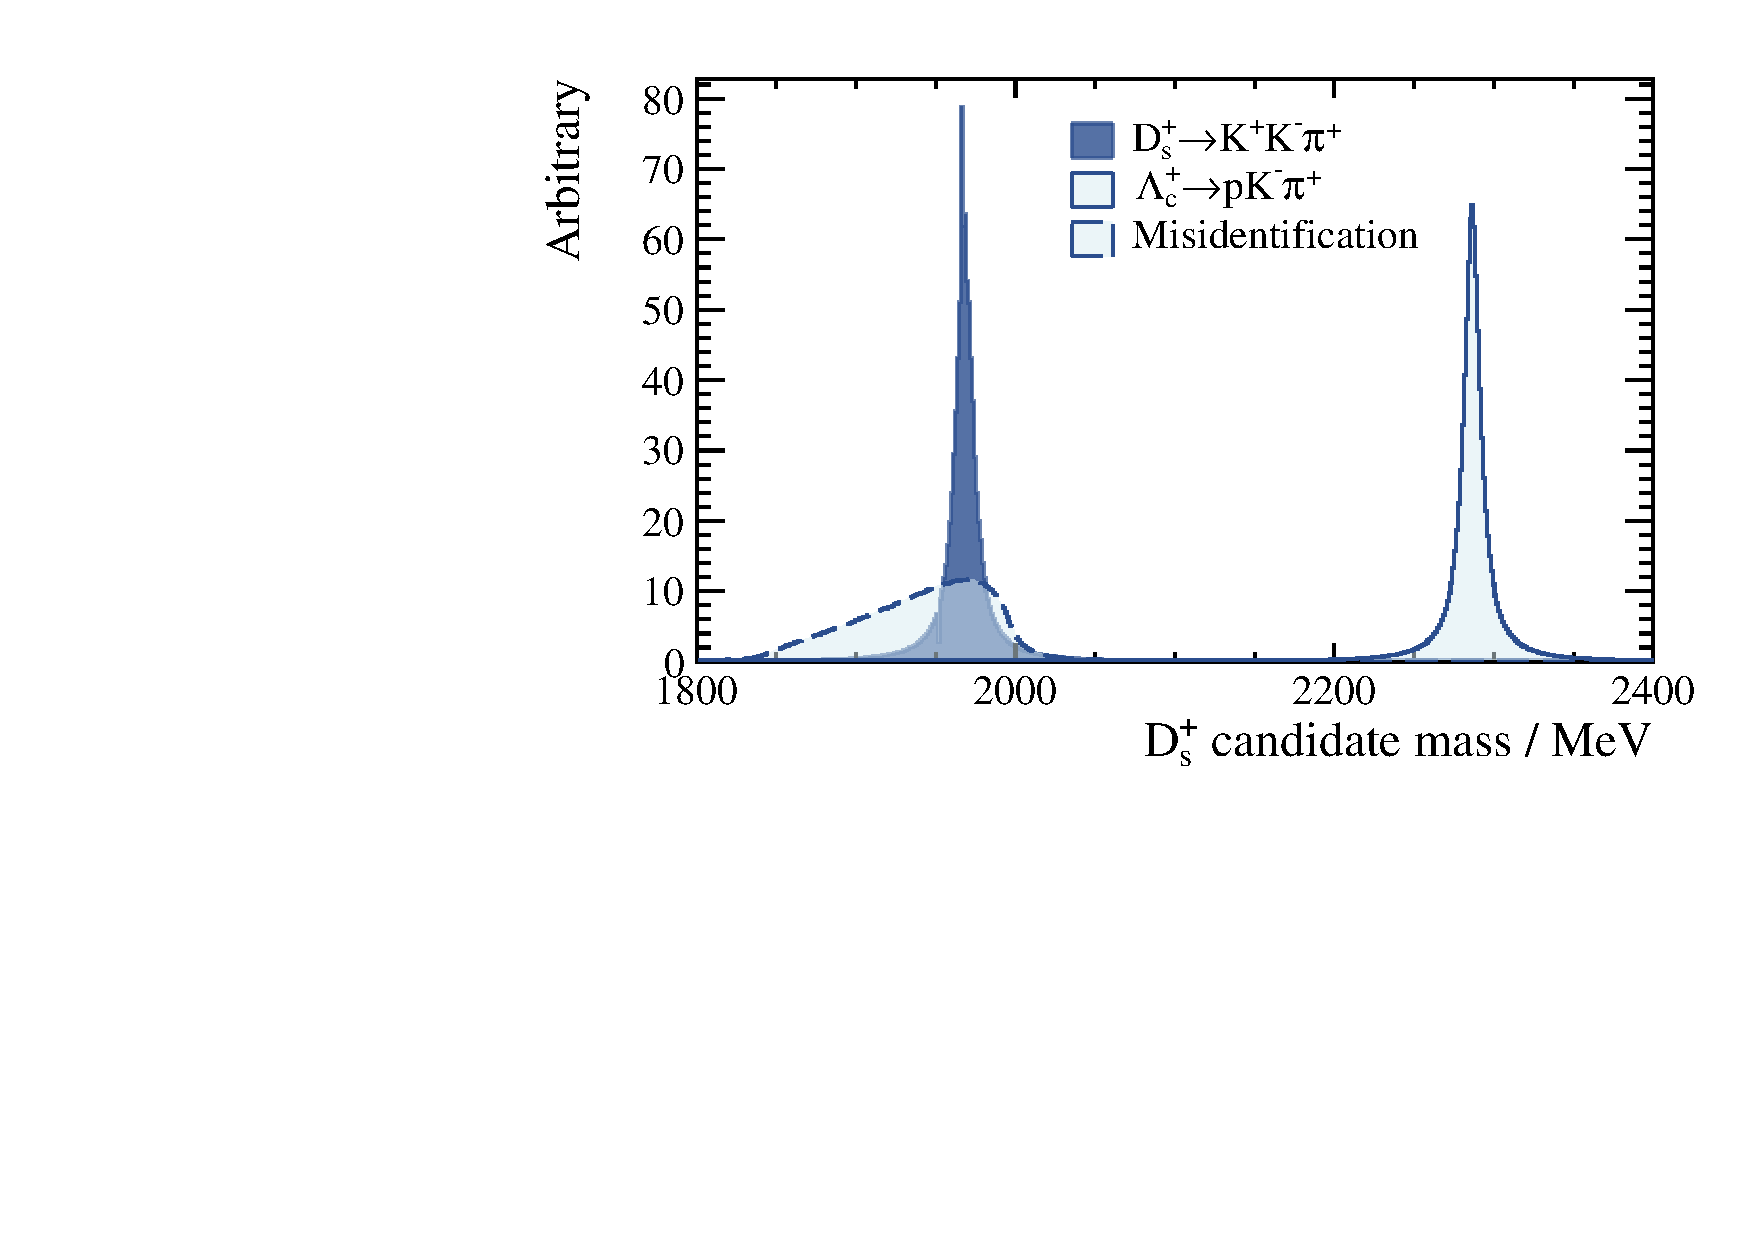
\includegraphics[width=0.48\textwidth]{tgen_lcveto}
    \caption{\small
      Simple phasespace simulations at generator level of the decay \decay{\Ds}{\kkpi}, along side
      (left) \decay{\Dp}{\kpipiss}, and
      (right) \decay{\Lc}{\pkpi},
      The distributions of the \Dp and \Lc decays, where one particle has been misidentified as a
      \Kp are also shown.
      Distributions after the misidentification are shown with a dotted outline, and sit under the
      \Ds mass peak.
      Each peak has the same integral.
    }
    \label{}
  \end{center}
\end{figure}




%These peaking backgrounds do not necessarily result in a longitudilnally polarized \phii.
%They are however, irriducible, and must be accounted for in the fit, this is described later in
%\Sec{sec:dsphi:fit}.

%In order to remove candidates from \Dp cross-feed,
%if the new $\Km\pip\pip$ mass falls within $25\mev$ of $m_{\Dp}^\pdg$,
%the kaon pair must either form an invariant mass within
%$10\mev$ of the known \phii mass, or the ambiguous track must pass stringent PID requirements
%($\dllkpi(\Kp)>10$).
%If the mass of the $p\Km\pip$ object falls within $25\mev$ of the \Lc mass,
%The candidate decay chain is then subject to the stripping requirements, which are outlined in
%\Tab{tab:dsphi:sel}.
%Requirements in the stripping are that the \Ds vertex is downstream of the \Bp and the vertices are
%well defined.
%One variable listed in \Tab{tab:dsphi:sel} is $\bdt_\mathrm{strip}$, which is the output of a BBDT
%in the stripping, whose input variables are a few kinematic and geometric variables of the \Bp and
%\Ds.
%The cut on this BBDT is very loose, and is approximately 100\pc efficient
%The \decay{\Ds}{\kkpi} and \decay{\phi}{\kk} candidates are required to have invariant masses
%within 25 and $20\mev$ of their known masses~\cite{PDG2012} respectively.



\subsection{Boosted Decision Tree}
Separation of \Ds and \phii candidates from the combinatorial background is done using a pair of
BDTs, one each to identify the decays \decay{\Ds}{\kkpi} and \decay{\phi}{\kk}.
The technique of using two different BDTs is also used in \decay{B}{DD} decays in
\Ref{LHCb-CONF-2012-009}.
%Each BDT was trained using the bagging method, as described in \Sec{sec:bdt:bag}.
%The signal and background data used to train these BDTs came entirely from data.
%Signal samples came from the decays $\decay{\Bbar^0_{s}{\Ds\pim}$ and $\decay{\Bs}{\jpsi\phi}$
%data, which was background subtracted by sWeighting~\cite{splot}.
%Background samples were taken from the sideband distributions of the same data.
%The BDT technique used in this analysis, also used in \Ref{LHCb-CONF-2012-009}, is different to
%other analyses in this thesis in that a BDT is trained for each the \Ds and $\phi$.
The boosting technique used here was bagging, which --- as described in \Sec{sec:bdt:bag} --- gives
a response in the range $0<\mathrm{BDT}<1$.
Cutting on the product of the two BDT responses improves the performance, and therefore the cut is
$\bdt_{\Ds}\times\bdt_\phi>X$, as opposed to $\bdt_{\Ds}>X_1$ and $\bdt_\phi>X_2$.

The BDT used to separate background from the signal \decay{\Ds}{\kkpi} decays was trained using
a signal sample of \decay{\Bs}{\Dsm\pip} sWeighted~\cite{splot} data, and background from the \Dsm
sidebands.
This BDT uses an unusually large array of training variables, given in \Tab{tab:dsphi:vars},
which include PID, and track quality variables.
In total, five variables are input for the parent \Ds and $\phi$, and 23 properties for each
daughter track.
Similarly for the \decay{\phi}{\kk} BDT, the signal sample was \decay{\Bs}{\jpsi\phi}, where
\jpsitomumu.


\begin{table}
  \caption[BDT variables]
  {\small
    List of training variables used in the \Ds and \phii BDTs.
    Each BDT uses five variables associated with the parent particle and 23 variables from each
    daughter track.
  }
  \label{tab:dsphi:vars}
  \begin{center}
    \begin{tabular}{clp{0.50\textwidth}}
      \toprule
      Particle & \multicolumn{2}{c}{Variable} \\
      \midrule
      \Ds, \phii
      & Kinematic variables & $p$, \pt \\
      & Geometric variables & \chisqvtx, \chisqip, \chisqfd \\
      \littlerule
      Tracks
      & Kinematic variables & $p$, \pt \\
      & Geometric variables & $\min(\chisqip)$ \\
      & Track variables     & 4 variables characterizing the track quality \\
      & PID variables       & 16 variables containing PID information, such as {\tt isMuon} and DLL
      variables from the \rich detectors \\
      \bottomrule
    \end{tabular}
  \end{center}
\end{table}


The cut for the BDT was optimized using the metric $S/\sqrt{S+B}$,
In this case, the number of signal events, $S$, was estimated from the yield from the decay
\decay{\Bs}{\Dsm\pip}, according to:
\begin{equation}
  S = \frac{ \BF\big(\btodsphi\big) }{ \BF\big(\bstodspi\big) }
  \frac{ \eff{geo}\big(\btodsphi\big) }{ \eff{geo}\big(\bstodspi\big) }
  \frac{f_d}{f_s}
  N\big(\bstodspi\big).
\end{equation}
Here, \eff{geo} is the geometric efficiency of the \lhcb detector, and $f_s/f_d$ quantifies
fraction of \Bs mesons produced relative to \Bd mesons.
The background yield is estimated as:
\begin{equation}
  B = c\cdot N_\mathrm{c}\big(\bstodspi\big)\cdot N_\mathrm{c}\big(\bstojpsiphi\big),
\end{equation}
where $N_\mathrm{c}$ indicates the yield of combinatoric background for a given decay, and
$c$ is a constant scaled such that
$N_\mathrm{c}\big(\bstodspi\big)\cdot
N_\mathrm{c}\big(\bstojpsiphi\big)=N_\mathrm{c}\big(\btodsphi\big)$ with no BDT cut.
The optimization procedure results in the optimal cut as $\bdt_{\Ds}\times\bdt_\phi>0.57$.



Invariant mass distributions of
selected candidate \Ds and \phii mesons are shown in \Fig{fig:dsphi:mesons}.

\begin{figure}
  \begin{center}
    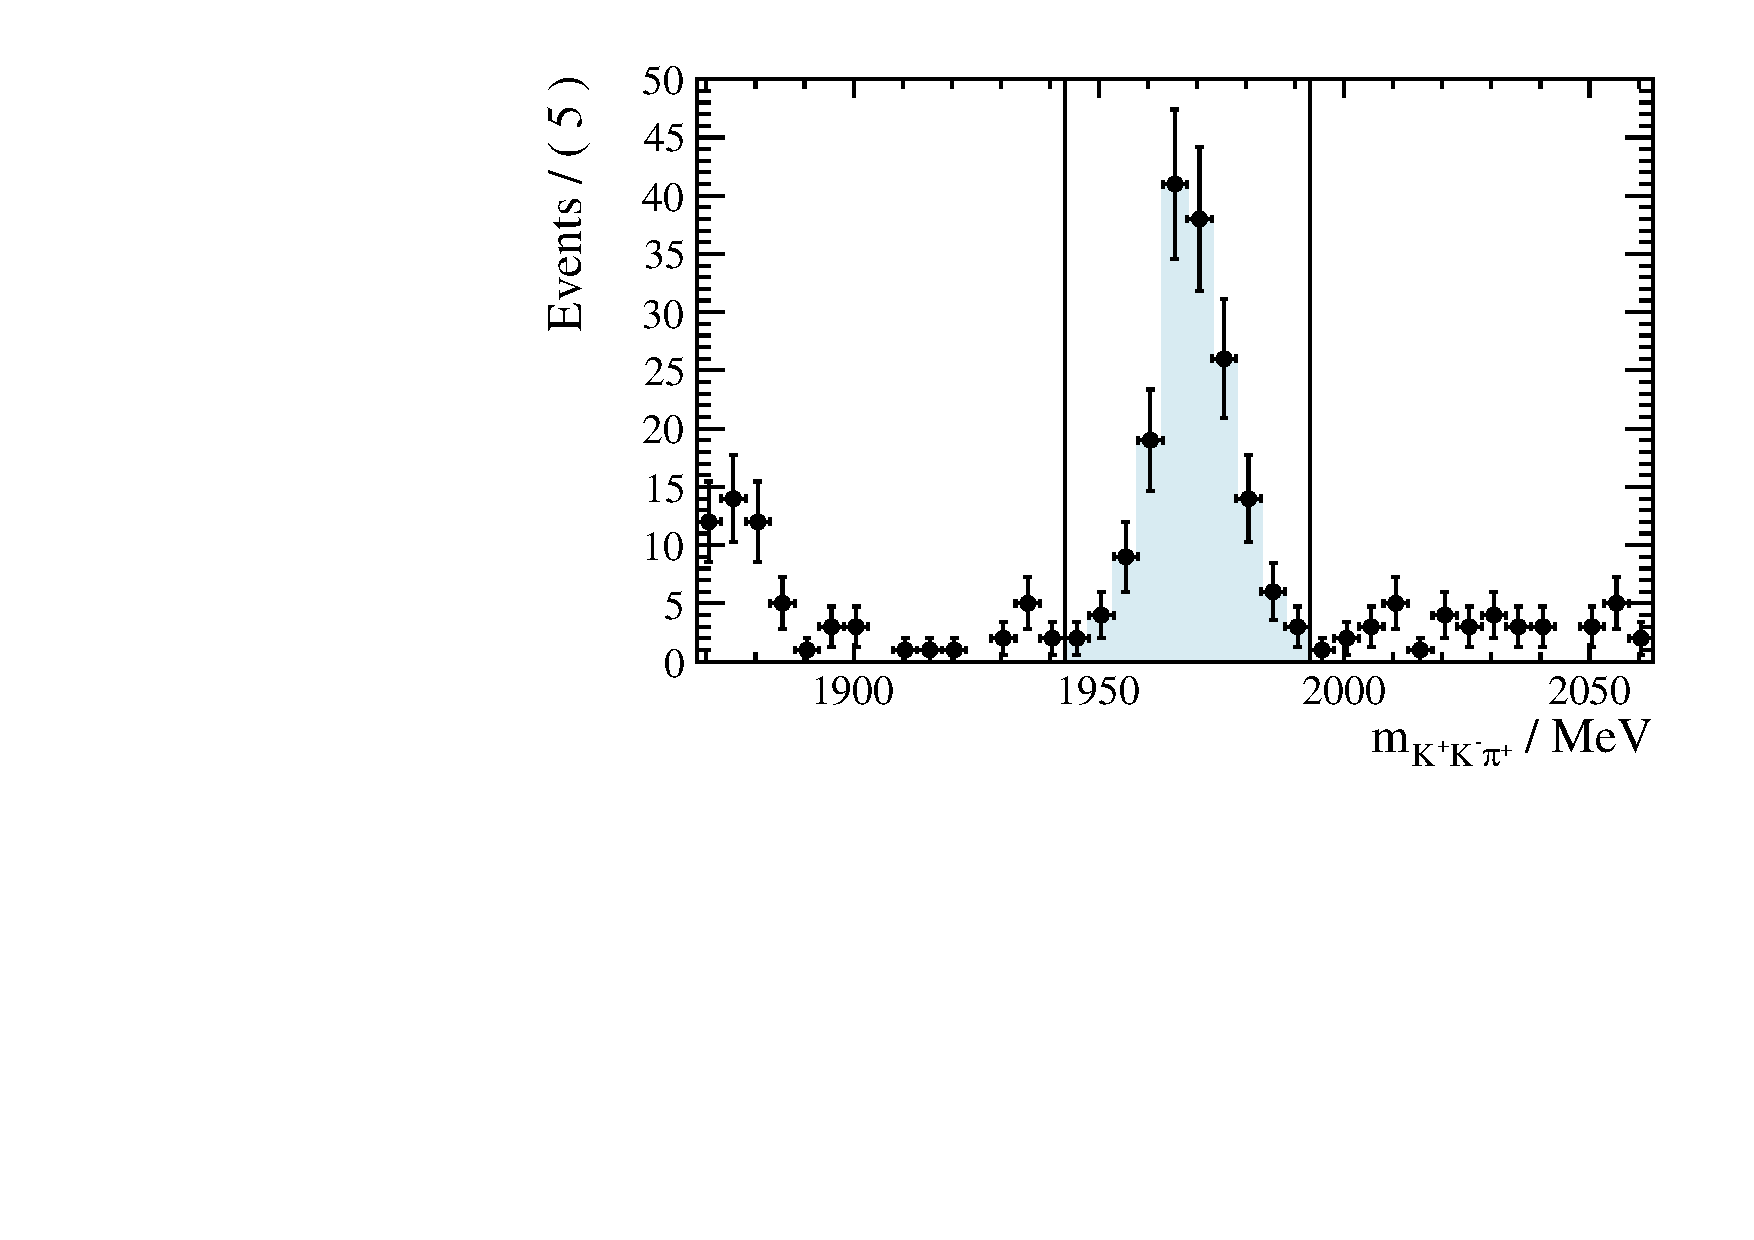
\includegraphics[width=0.48\textwidth]{spectrum_ds}
    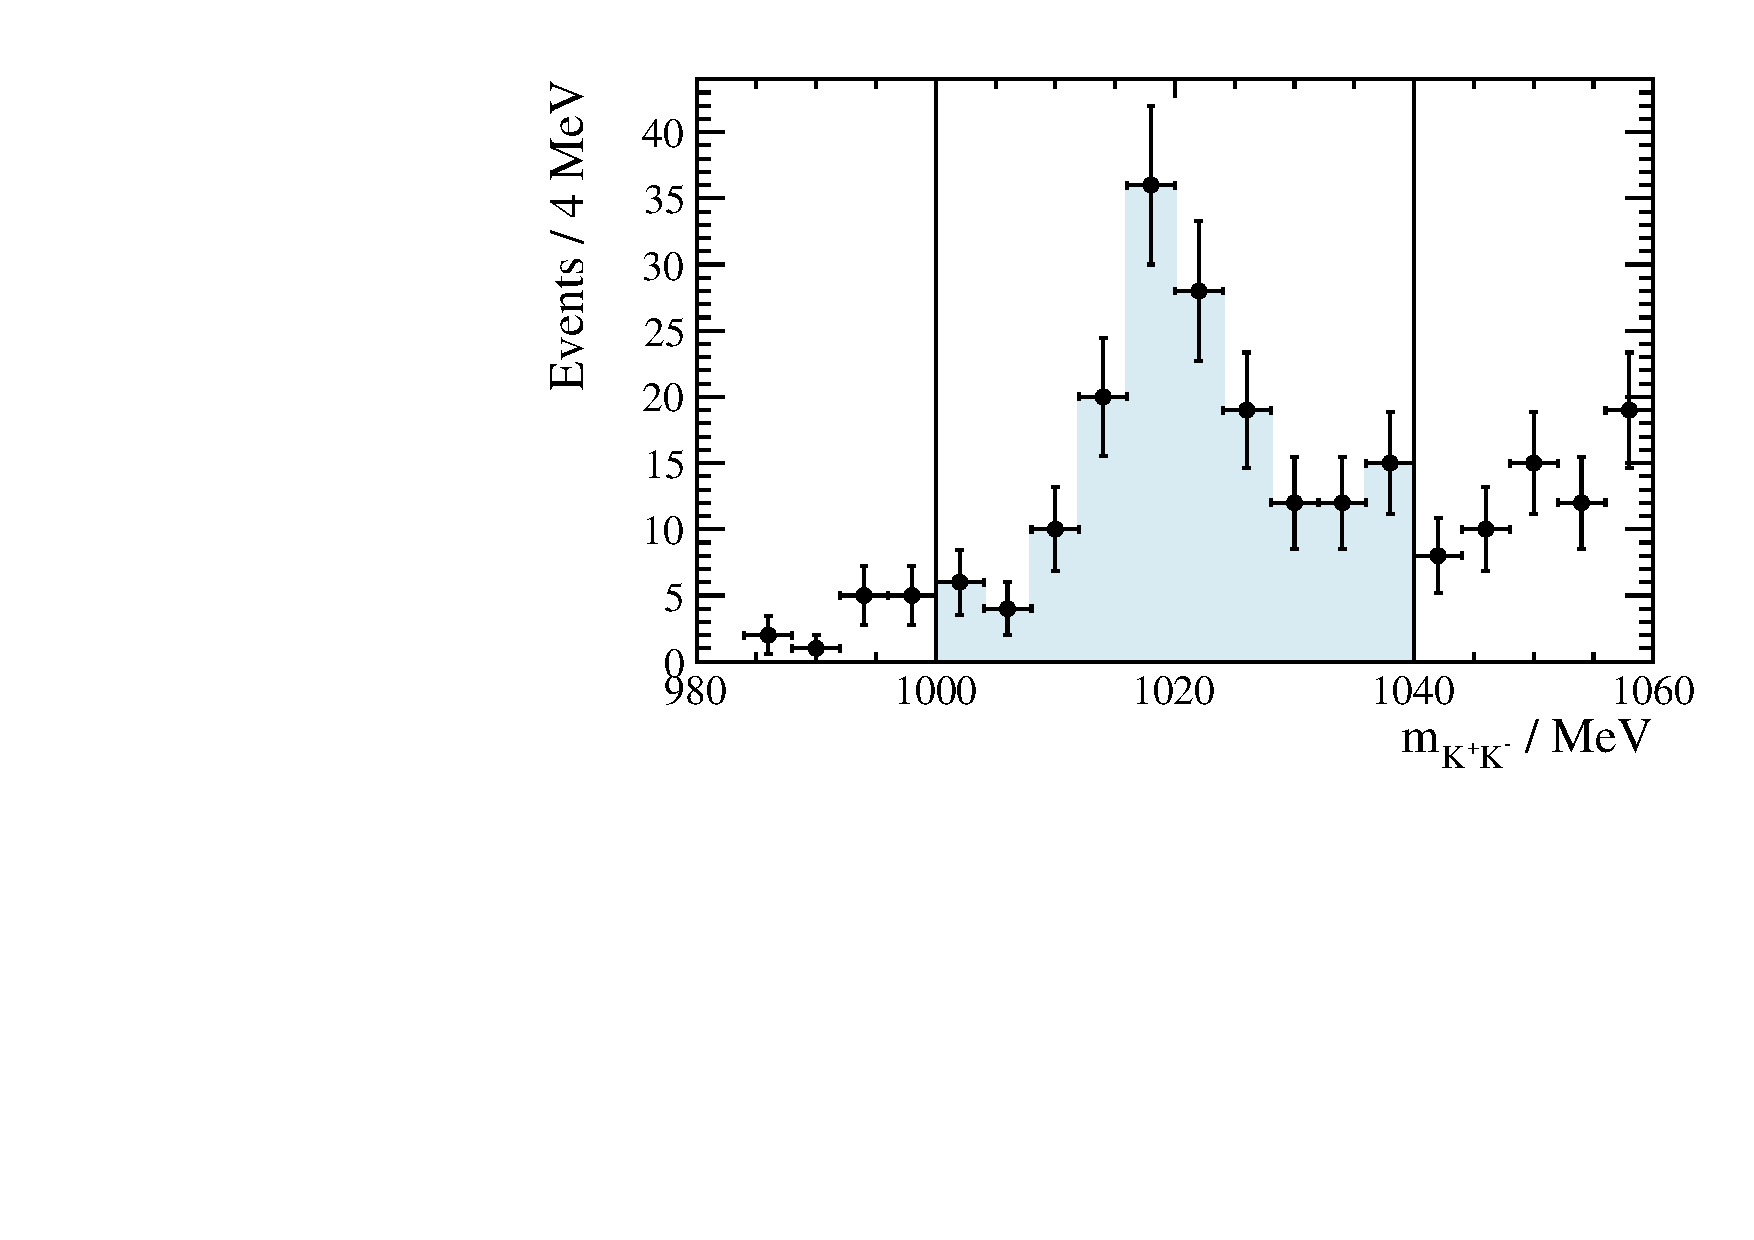
\includegraphics[width=0.48\textwidth]{spectrum_phi}
    \caption{\small
      Invariant mass distributions of the candidate
      (left) \decay{\Ds}{\kkpi}, and
      (right) \decay{\phii}{\kk} candidates.
      The \kkpi spectrum shows a range of masses, where the vertical black lines indicate the
      boundaries of the mass cut $|m_{\kkpi}-m_{\Ds}^\pdg|<25\mev$, where the shaded candidates are
      those that are accepted.
      On the far left of this distribution, a mass peak from \decay{\Dp}{\kkpi} is also visible.
      The \decay{\phi}{\kk} spectrum is shown in the range $|m_{\kk}-m_{\phi}^\pdg|<40\mev$,
      and the signal region is indicated by the vertical black lines and shaded data.
    }
    \label{fig:dsphi:mesons}
  \end{center}
\end{figure}






%\subsection{Fit regions}
%\label{sec:dsphi:hel}
%The final state particles in this analysis of the decay \btodsphi are $\kkpi\kk$, given the mass
%cuts on the \Ds and \phii candidates, there are no sources of background which peak at the \Bp
%mass.
%However, there are backgrounds from genuine $B$-hadron decays in which a particle --- or multiple
%particles --- are not reconstructed.
%These backgrounds form below the mass of the \Bp.
%After the selection requirements
%%There are no backgrounds which contribute to a peaking component directly below the \Bp mass for
%%the decay \btodsphi.
%%However, on top of the combinatorial background, the low-mass side has a number of components which
%%result from excited \Dssp or \Kstarz.
%The most significant of these are the decays\footnote{
  %For these decays the \Kstarz refers to the $K^*(892)^0$ meson.
%}
%\btodsstrphi, \bstodskstrk and \bstodsstrkstrk.
%%which all contain at least one final state particle that is not reconstructed.

%The decay \bstodskstrk has never been observed, but given that the branching fraction of the decay
%$\decay{\Bd}{\Dm\Kstarzb\Kp}$ is $(8.8\pm1.9)\e{-4}$~\cite{PDG2012}, it should be in the
%\btodsphi selection.
%There is no contribution from the \decay{\Bd}{\Dm\Kstarzb\Kp} mode, because the loss in mass from
%the pion means that it peaks too low.
%As well as this, the decay \bstodsstrkstrk was also expected to be present in the sample, though at
%lower mass.



%A \Bp meson has quantum numbers $J^P=0^-$, and the \Ds and $\phi$ mesons have
%quantum numbers $0^-$ and $1^-$ respectively.
%Therefore the decay \btodsphi is a transition of a pseudoscalar to a pseudoscalar and a vector
%meson.
%In order for angular momentum to be conserved, the vector particle must be produced in the $j=0$
%state, where the spin is orthogonal to the particle's momentum.
%The $\phi$ is the vector meson in the decay \btodsphi, in its final state it is lonitudinally
%polarized, and its daughter kaons have an angular distribution proportional to $\cos^2\thetahel$;
%where \thetahel is the helicity angle, defined as the angle between the \Kp and the \Bp in the rest frame of the \Ds.
%This fact is used to further separate the signal decay \btodsphi from other backgrounds.


%It is possible to remove about $93\pc$ of background by requiring that $|\cos\thetahel|>0.4$,
%this is the same cut value as used in \Ref{LHCb-PAPER-2011-008}.
%Therefore, two regions are defined in terms of $\cos\thetahel$, and both are used in a simultaneous
%fit.
%This also allows the combinatorial and peaking backgrounds to be separated from the signal because
%these do not necessarily have a longitudilnally polarized \phii.

%%The signal region for the \phii candidate is defined to be within $20\mev$ of $m_\phii^\pdg$.
%%A sideband region is defined to be $20<m_

%%These peaking backgournds, and the combinatorial background,
%%do not have to have a $\phi$ meson in a longitudilnally polarized.
%%Therefore, the $\cos\thetahel$ distribution should be flat for all backgrounds.

%%can be used to separate the signal decay from backgrounds.

%%In order to maximize the signal yield, the full selected dataset was separated into four regions
%%defined by the helicity angle and the invariant mass of the $\phi$ candidate, these regions are
%%shown in \Table{tab:dsphi:hel}.

%Fit regions are further split according to the invariant mass of the \phii candidate.
%A signal region is defined for \phitokk candidates with a mass within $20\mev$ of the nominal \phii
%mass, and a sideband region is defined for candidates with a mass in the range
%$20<m_\phi^\pdg<40\mev$.

%The resulting fit regions --- defined by \thetahel and $m_{\kk}$ --- have a signal region, \rA,
%containing most of the signal, and a purely background region, \rD.
%By performing a simultaneous fit to the four regions, which are defined explicitly in
%\Tab{tab:dsphi:hel}, there is a better grasp on all the backgrounds.

%\begin{table}
  %\caption[Fit regions]
  %{\small
    %Fit regions used to search for the decay \btodsphi.
    %Approximately $89\,\%$ was expected to be in region \rA.
  %}
  %\label{tab:dsphi:hel}
  %\begin{center}
    %\begin{tabular}{cccc}
      %\toprule
      %&&\multicolumn{2}{c}{$|m_{KK}-m_\phi^\pdg|$ (MeV)}\\
      %&&$\in[0,20]$&$\in[20,40]$ \\
      %\midrule
      %\multirow{2}{*}{$|\cos\thetahel|$}
      %&$>0.4$ & \rA & \rB \\
      %&$<0.4$ & \rC & \rD \\
      %\bottomrule
    %\end{tabular}
  %\end{center}
%\end{table}





